\documentclass{article}

\usepackage{graphicx}
\usepackage{tikz}
\usepackage{tikzsymbols}
\usetikzlibrary{calc,patterns,shapes.geometric}
\pagestyle{empty}
\usepackage[margin=0pt]{geometry}
\geometry{papersize={14in,12in}}

\def\centerarc[#1](#2)(#3:#4:#5){\draw[#1] ($(#2)+({#5*cos(#3)},{#5*sin(#3)})$) arc (#3:#4:#5);}

\begin{document}
	\begin{figure}
		\centering
		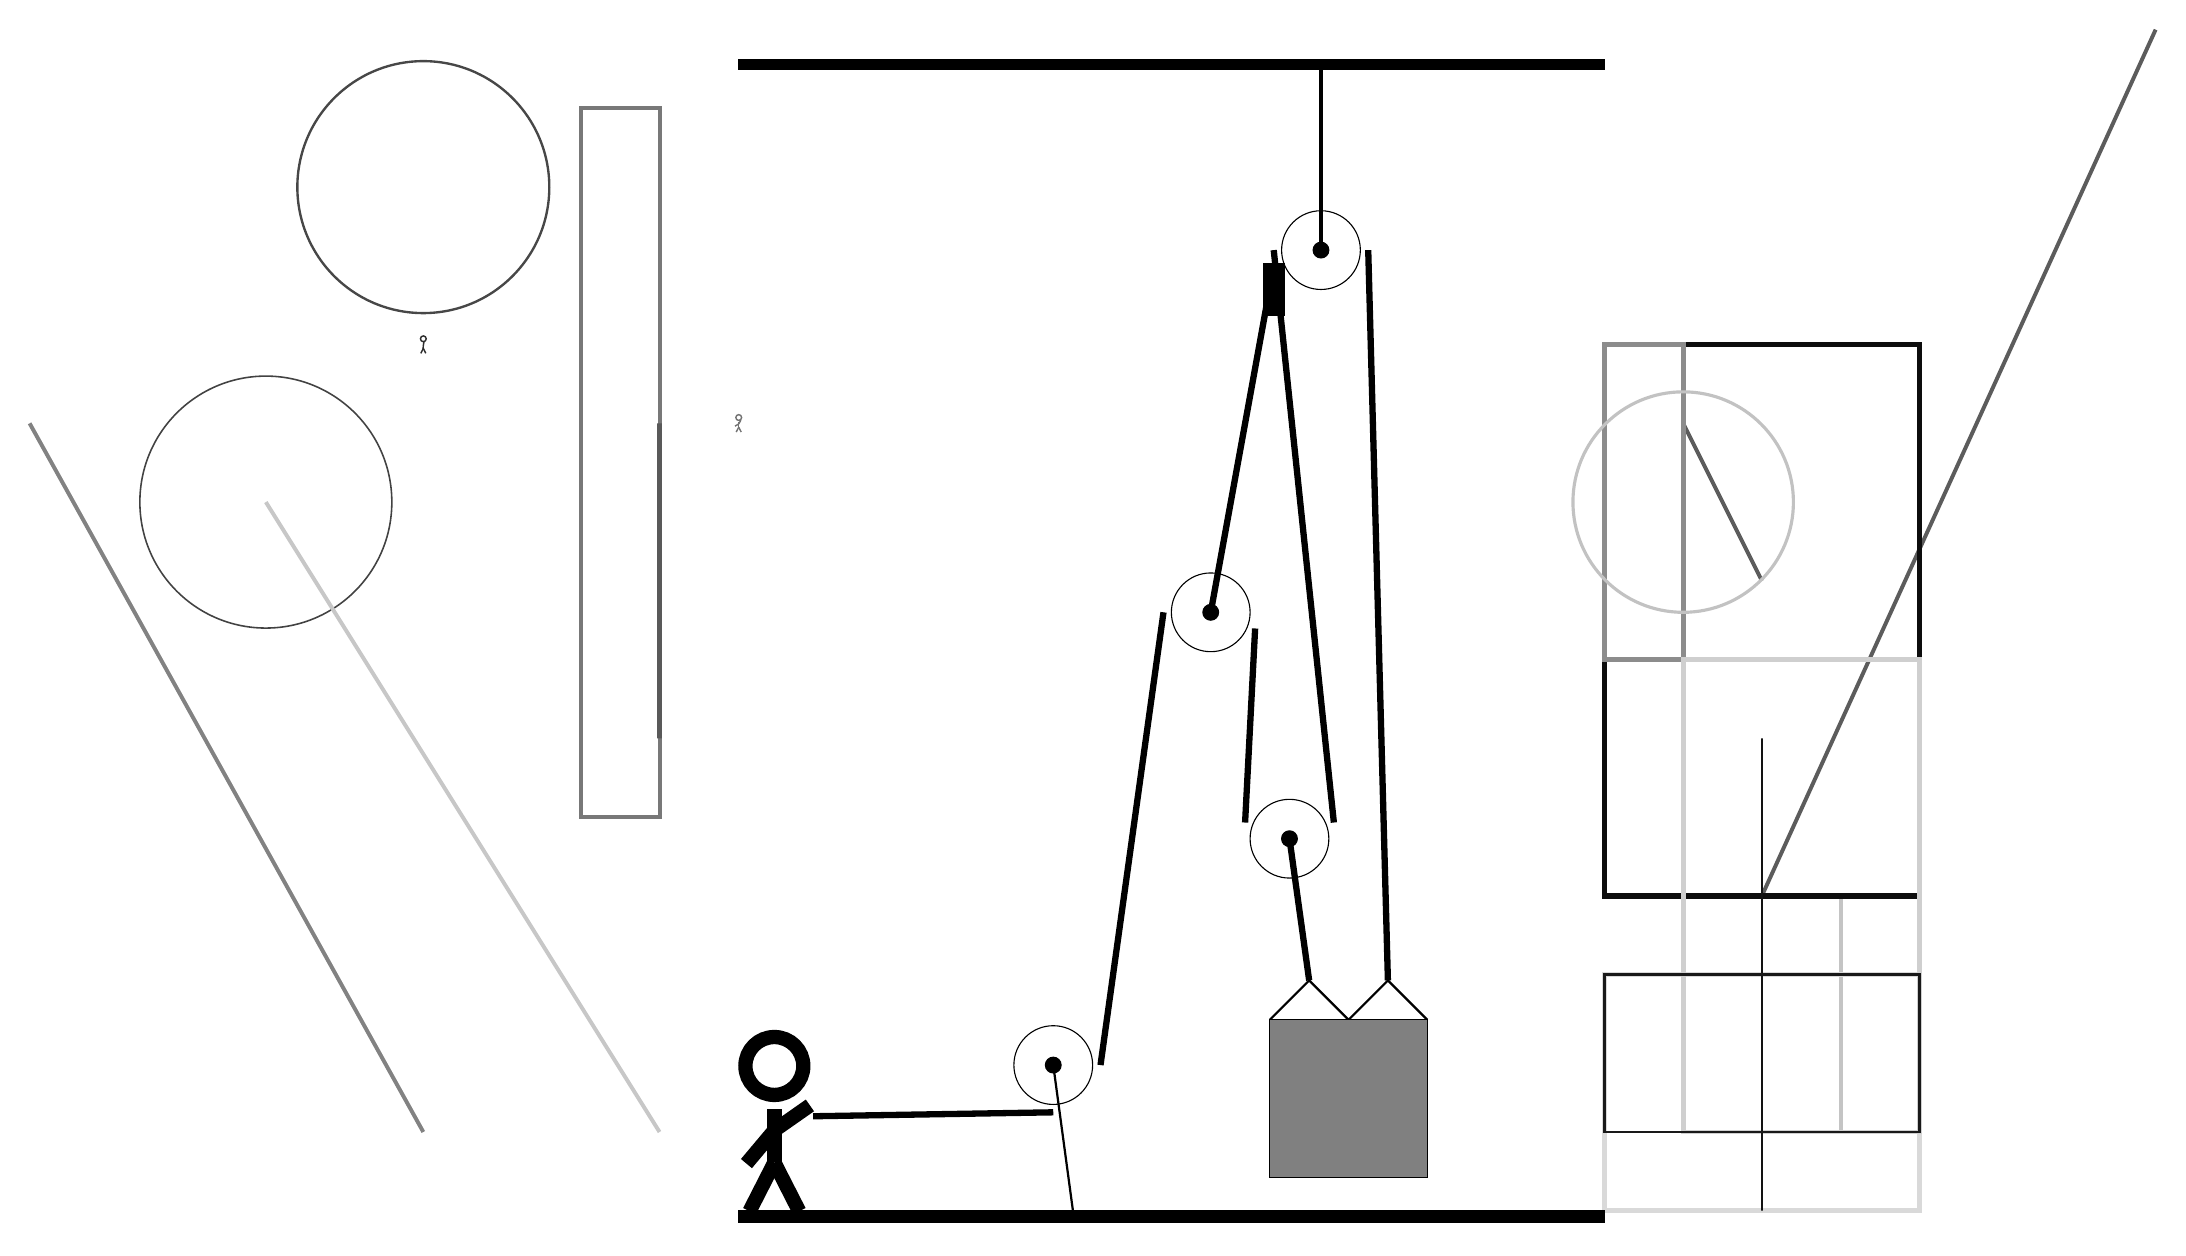
\begin{tikzpicture}
			%%%%% START %%%%%
			
			\draw[fill=black] (-6, 11.5) rectangle (5, 11.625);
			
			\draw (0, 4.6) circle (0.5);
			\draw[fill=black] (0, 4.6) circle (0.1);
			
			\draw (1, 1.725) circle (0.5);
			\draw[fill=black] (1, 1.725) circle (0.1);
			
			\draw (1.4, 9.2) circle (0.5);
			\draw[fill=black] (1.4, 9.2) circle (0.1);
			\draw[very thick] (1.4, 9.2) -- (1.4, 11.5);
			
			\draw (-2, -1.15) circle (0.5);
			\draw[fill=black] (-2, -1.15) circle (0.1);
			\draw[thick] (-2, -1.15) -- (-1.75, -3);
			
			
			\draw [line width=0.2mm, color=black!74](-12, 6) circle (1.6);
			
			\draw[line width=0.5mm, color=black!64](7, 1) -- (12, 12);
			\draw[line width=0.5mm, color=black!23](8, 1) -- (8, -2);
			\node[line width=0.5mm, color=black!55] at (-6, 7) {\Strichmaxerl[1][30][61]};
			
			\draw[line width=0.7mm, color=black!95] (5, 1) rectangle (9, 8);
			
			\draw[line width=0.5mm, color=black!64](6, 7) -- (7, 5);
			
			\draw[line width=0.5mm, color=black!22](-7, -2) -- (-12, 6);
			\draw[line width=0.5mm, color=black!53] (-8, 2) rectangle (-7, 11);
			\draw[line width=0.6mm, color=black!45] (5, 4) rectangle (6, 8);
			
			\draw[line width=0.6mm, color=black!15] (5, 0) rectangle (9, -3);
			\draw[line width=0.6mm, color=black!19] (6, -2) rectangle (9, 4);
			\node[line width=0.3mm, color=black!82] at (-10, 8) {\Strichmaxerl[1][86][79]};
			\draw[line width=0.3mm, color=black!93] (7, 3) rectangle (7, -3);
			
			\draw [line width=0.4mm, color=black!24](6, 6) circle (1.4);
			\draw [line width=0.3mm, color=black!72](-10, 10) circle (1.6);
			\draw[line width=0.3mm, color=black!90] (5, -2) rectangle (9, 0);
			
			\draw[line width=0.6mm, color=black!65] (-7, 7) rectangle (-7, 3);
			\draw[line width=0.5mm, color=black!49](-10, -2) -- (-15, 7);
			
			\draw[thick]  (0.75, -0.575) -- (1.25, -0.075) -- (1.75, -0.575) -- (2.25, -0.075) -- (2.75, -0.575);
			\draw[fill=black!50] (0.75, -0.575) rectangle (2.75, -2.575);
			\draw[line width=0.8mm] (-5.05, -1.8) -- (-2, -1.75);
			\centerarc[line width=0.8mm](-2, -1.15)(270:360:0.6);
			\draw[line width=0.8mm] (-1.4, -1.15) -- (-0.6, 4.6);
			\draw[line width=0.8mm] (0, 4.6) -- (0.8, 9.0);
			\draw[line width=0.8mm, fill=black](0.7, 8.4) rectangle (0.9, 9.0);
			\centerarc[line width=0.8mm](0, 4.6)(-20:180:0.6);
			\draw[line width=0.8mm] (0.5638, 4.3948) -- (0.4362, 1.9302);
			\centerarc[line width=0.8mm](1, 1.725)(160:380:0.6);
			\draw[line width=0.8mm] (1.5638, 1.9302) -- (0.8, 9.2);
			\draw[line width=0.8mm](1, 1.725) -- (1.25, -0.075);
			\centerarc[line width=0.8mm](1.4, 9.2)(0:180:0.6);
			\draw[line width=0.8mm] (2.0, 9.2) -- (2.25, -0.075);
			
			\node at (-5.5, -1.9) {\Strichmaxerl[10][50][35]};
			
			\draw[fill=black] (-6, -3) rectangle (5, -3.15);
			
			%%%%% END %%%%%
		\end{tikzpicture}
	\end{figure}	
\end{document}